\begin{figure}[!htb]
  \centering
  \caption{Dynamic Moments (Myopia)}
  \begin{minipage}[t]{0.4\textwidth}
    \centering
    \small{(a) Earnings}
    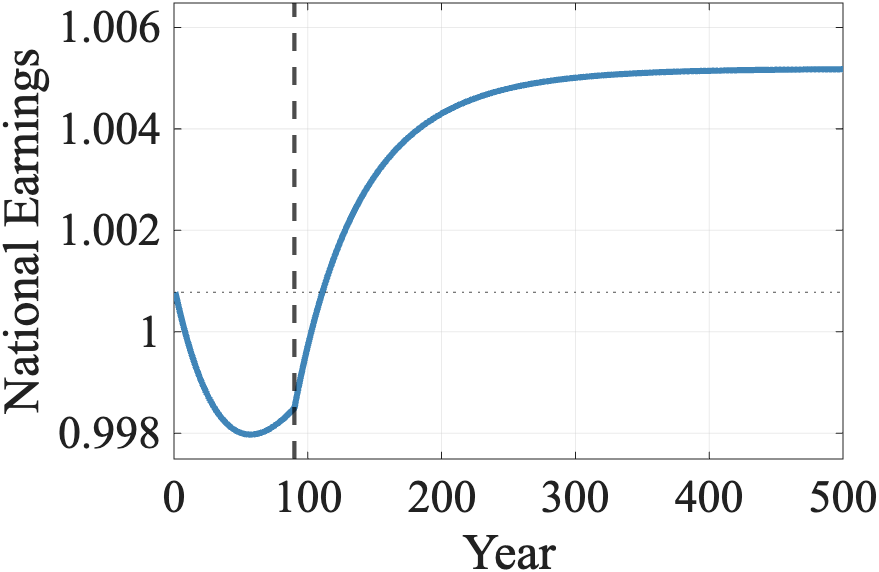
\includegraphics[width=\textwidth]{../Output/big_nu/graph_myopia/dynamic_moments/dynamic_moments_national_earnings.png}
  \end{minipage}\hfill
  \begin{minipage}[t]{0.4\textwidth}
    \centering
    \small{(b) Mobility}
    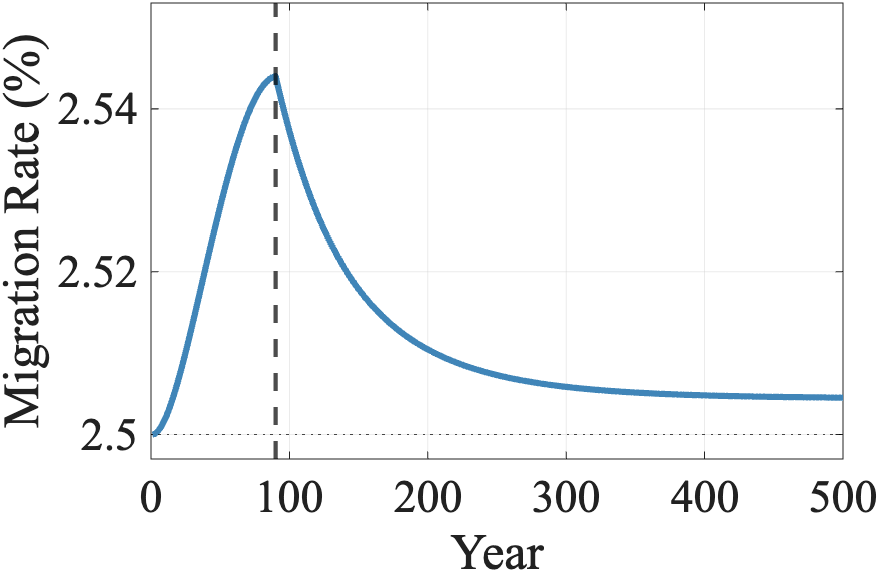
\includegraphics[width=\textwidth]{../Output/big_nu/graph_myopia/dynamic_moments/dynamic_moments_national_mobility.png}
  \end{minipage} \\[2ex]
  \begin{minipage}[t]{0.4\textwidth}
    \centering
    \small{(c) Wealth}
    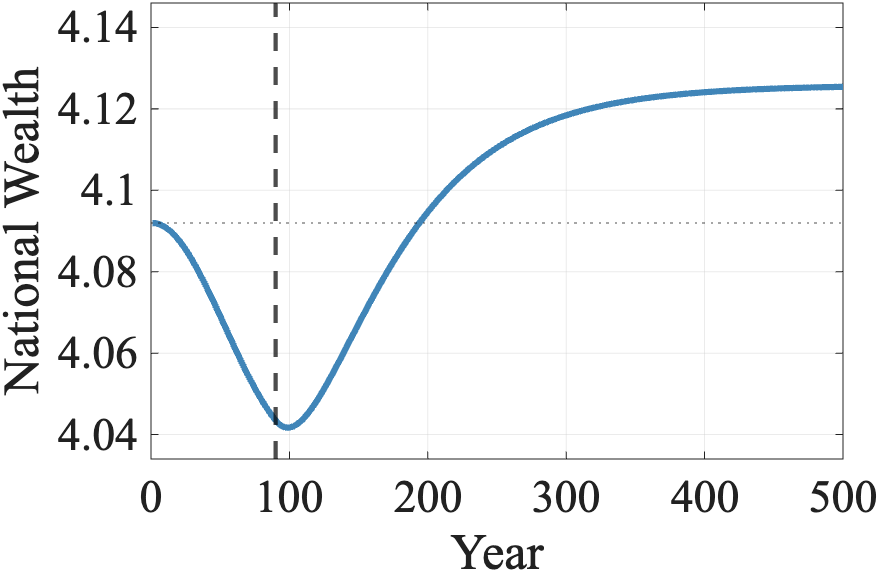
\includegraphics[width=\textwidth]{../Output/big_nu/graph_myopia/dynamic_moments/dynamic_moments_national_wealth.png}
  \end{minipage}\hfill
  \begin{minipage}[t]{0.4\textwidth}
    \centering
    \small{(d) W/Y Ratio}
    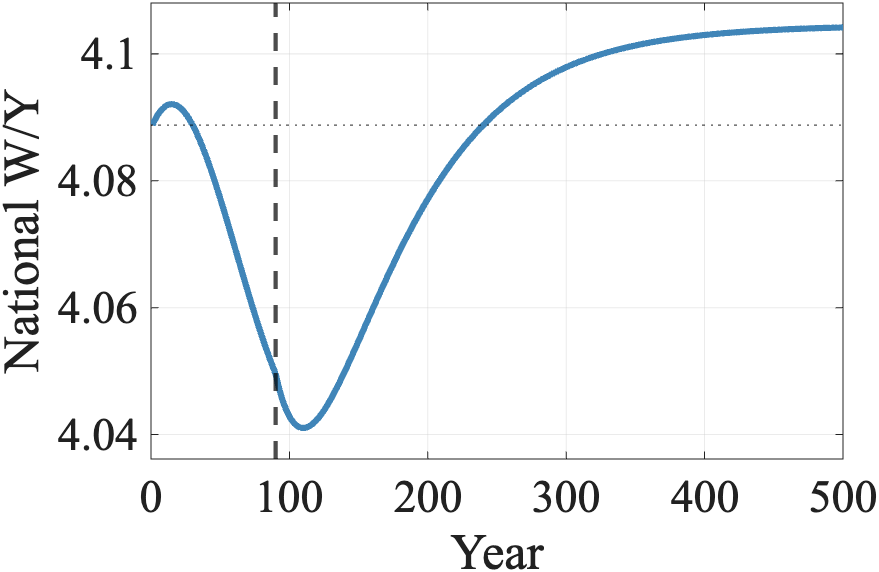
\includegraphics[width=\textwidth]{../Output/big_nu/graph_myopia/dynamic_moments/dynamic_moments_national_wy.png}
  \end{minipage}
  \begin{minipage}{\textwidth}
  \vspace{0.5em}
  \footnotesize{\textbf{Note:} Aggregate macroeconomic time series under Myopia, 2010--2500+. Agents optimise assuming current parameters persist indefinitely, solving value indices $\boldsymbol{\Xi}_t^{\text{myopia}}$ as static fixed points at each period $t$ without backward induction. Panel (a): national total disposable earnings $Y_t = \sum_{\ell,z} \tilde{w}_{\ell,t} (L_{\ell,t} + z \Lambda_t(\ell,z))$. Panel (b): national gross annual migration rate $m_t = \sum_{\ell,z} \Lambda_t(\ell,z) [1 - \mu_{\ell \ell,t}(z)] / \sum_\ell L_{\ell,t}$. Panel (c): national wealth mass $W_t = \sum_{\ell,z} \bar{a}_t(\ell,z) \Lambda_t(\ell,z)$. Panel (d): wealth-to-earnings ratio $(W/Y)_t = W_t / Y_t$.} \end{minipage}
  \label{fig:trans_dyn_myopia}
\end{figure}